\chapter{General Introduction}
\newpage
\section{Prologue}
The oceans constitute a fundamental component of the Earth system, being intrinsically linked to a wide range of physical and biogeochemical processes. They play a central role in the global climate by absorbing the majority of the excess heat and redistributing it through ocean circulation \parencite{vonschuckmann2023heat}. Ocean-atmosphere interactions strongly influence weather patterns, including the distribution of precipitation, the occurrence of droughts, and the intensity of extreme events such as floods and storms \parencite{seo2023ocean, chen2024analysis}. Beyond their climatic significance, the marine environment supports an extraordinary diversity of life, hosting complex ecosystems that are essential for global biodiversity \parencite{talukder2022climate, ipcc2022changing}. From a socio-economic perspective, the oceans contribute to global food security and livelihoods \parencite{free2022expanding}, serving as a key medium for transportation and international trade, and underpinning tourism and cultural practices \parencite{jouffray2020blue}. Their economic importance also extends to the exploitation of natural resources, including fossil fuels, minerals, and renewable energy \parencite{oecd2016ocean}.

Understanding the mechanisms that govern ocean dynamics is therefore essential for promoting the sustainable use of marine resources and for addressing pressing environmental challenges, particularly those associated with climate change. In this context, continuous monitoring of the ocean becomes a fundamental requirement for advancing scientific knowledge, and is primarily achieved through two complementary approaches: ocean observation and numerical modelling. The systematic acquisition, processing, and dissemination of ocean data within this framework are encompassed by the concept of operational oceanography, which aims to provide regular and reliable information on the state of the ocean \parencite{fanjul2024promoting, serafy2023eurogoos}.

Observation systems provide valuable insights into ocean variability and long-term changes in water properties across multiple variables, such as ocean temperature, acidification, and sea-level rise \parencite{frederikse2020causes, vonschuckmann2025global}. On the other hand, numerical models help overcome the inherent limitations of observations by filling spatial and temporal gaps and supporting a wide range of operational and environmental applications, including the simulation of past conditions (hindcast) (e.g., \textcite{sasaki2020global}), forecasting \parencite{cima2024soma}, oil-spill dispersion \parencite{janeiro2017integrating}, and marine litter transport \parencite{rosas2022pathways}, among others. As these two approaches are inherently complementary, observation data can be integrated into model simulations in a statistically consistent manner. In this context, data assimilation (DA) methodologies can effectively combine observations and model outputs while accounting for their respective uncertainties. Through this integration, DA produces improved estimates of the ocean state, yielding a more accurate and dynamically consistent representation of marine systems \parencite{martin2025data, carrassi2018data}.

\section{Ocean Observation}
The primary focus of this dissertation is not to provide a detailed description of ocean observation methods and systems. However, as these are extensively referenced throughout the following chapters, it is important to briefly outline the main approaches used to monitor the ocean. According to \textcite{miguez2026goos}, the key variables required to effectively understand the oceans are defined as Essential Ocean Variables (EOVs), which provide a standardized framework for guiding global ocean observation efforts. These variables are typically grouped into three main categories: physical EOVs, which include temperature, salinity, sea level, currents, and waves; biogeochemical EOVs, such as dissolved oxygen and nutrients; and biological and ecosystem EOVs, including indicators such as phytoplankton biomass and fish abundance.

Regardless of the variable of interest, ocean data are fundamentally collected through two complementary methods: \emph{in situ} measurements, obtained directly within the marine environment, and remote sensing, primarily based on satellite observations. The operational network of \emph{in situ} instruments is complex and requires significant coordination and sustained effort, as maintaining adequate spatial and temporal coverage is essential to minimize observational gaps \parencite{legler2015current}. The most common \emph{in situ} observational platforms are outlined below.

\emph{Surface drifters}

Surface drifters are Lagrangian observing platforms that follow ocean currents and provide direct measurements of upper-ocean circulation. They are widely used to study ocean dynamics, transport processes, and variability, as well as to support and validate numerical models \parencite{lee2025surface}.

\emph{Argo profiling floats}

The Argo program is one of the most important operational ocean observing networks for global ocean monitoring, implemented through a coordinated multinational effort involving numerous countries. It is composed of thousands of autonomous profiling floats (\bCref{fig:argo_1.1}) that operate on repeated cycles, drifting at depth before descending and subsequently ascending through the water column to collect vertical profiles of temperature, salinity, and pressure \parencite{thierry2025advancing}. The data is then transmitted in near-real time via satellite, when the floats are at the surface. More recent developments include the integration of biogeochemical sensors measuring variables such as dissolved oxygen, acidity, nitrate, and chlorophyll, significantly expanding the scope of ocean monitoring.

\begin{figure}[H]
    \centering
    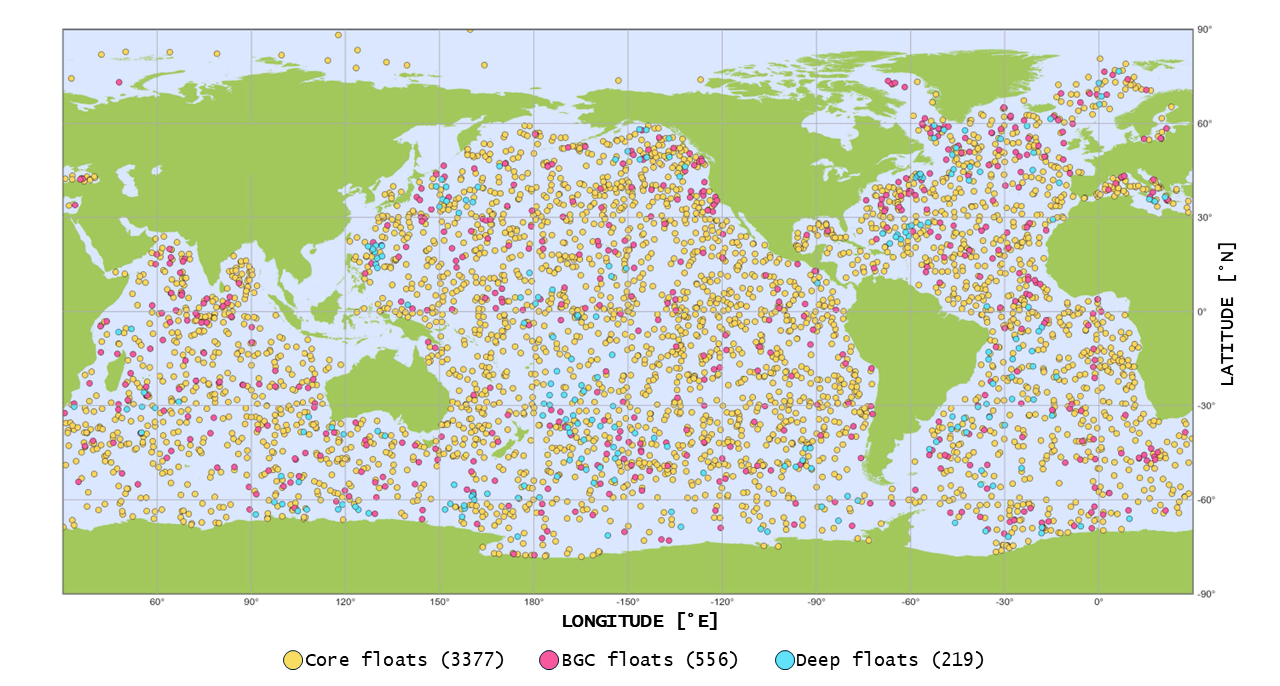
\includegraphics[width=16.0 cm]{figures/fig1.1.png}
    \caption{Global spatial distribution of Argo float deployments as of March 2025. The network includes three main types of profiling floats: Core floats, which measure temperature, salinity, and pressure in the upper 2000 m of the ocean; biogeochemical (BGC) floats, which are additionally equipped with sensors to observe variables such as dissolved oxygen, acidity, nitrate, and chlorophyll; and Deep floats, designed to extend observations to depths greater than 2000 m, reaching up to 4000-6000 m depending on the platform. The numbers in parentheses indicate the total number of active floats of each type. \emph{Source: adapted from \textcite{thierry2025advancing}}.}
    \label{fig:argo_1.1}
\end{figure}

\emph{Expendable bathythermograph (XBT) probes}

XBTs are widely used oceanographic instruments that provide vertical profiles of seawater temperature. Measurements are obtained through a thermistor embedded in a free-falling probe, while depth is estimated indirectly from a fall-rate equation rather than measured directly \parencite{simoncelli2024reprocessing}. The probe is not recovered after deployment.

\emph{Research vessels}

Despite being large and resource-intensive platforms, research vessels are highly specialized for oceanographic applications. They enable the collection of water samples for biogeochemical analysis and the deployment of complex and heavy instrumentation \parencite{satterthwaite2025essential}. While they remain fundamental to ocean research, ship-based observations are typically episodic and campaign-based rather than continuously operational.

\emph{Gliders and autonomous underwater vehicles (AUVs)}

Underwater gliders and AUVs are mobile robotic platforms designed to follow predefined mission trajectories and collect oceanographic data. AUVs use propeller-based propulsion systems that enable active control of their movement \parencite{sahoo2019advancements}, whereas gliders rely on buoyancy-driven motion combined with hydrodynamic lift generated by wings \parencite{wang2025development}. These platforms typically perform repeated vertical profiles, following a sawtooth trajectory, to acquire measurements of physical and, in some cases, biogeochemical variables throughout the water column. Despite their versatility, their operation is constrained by factors such as energy consumption, endurance, and depth limitations.

\emph{Commercial or non-research vessels}

Ship-based observing systems, including Ships of Opportunity (SOOP) and Volunteer Observing Ships (VOS), rely primarily on commercial vessels equipped with sensors to collect oceanographic and atmospheric data during routine operations. These platforms provide cost-effective observations with broad spatial coverage and play a key role in sustaining operational XBT deployments \parencite{haris2021sounding, jiang2019enhancing}. However, their sampling is often constrained by predefined shipping routes, which may not coincide with regions of specific scientific interest.

\emph{Moorings}

Moorings are typically fixed platforms equipped with multiple sensors that provide high temporal resolution time series of a wide range of oceanographic properties. They can collect measurements throughout the water column at a fixed location, as well as atmospheric variables at the surface. In addition to physical parameters, moorings can be instrumented to measure biogeochemical variables such as oxygen, carbon dioxide, and chlorophyll \parencite{bailey2019coastal}. Due to their relatively high installation and maintenance costs, moorings are deployed in limited numbers and are generally located in regions of particular scientific or operational interest.

\emph{High-frequency radar (HFR)}

HFR systems, typically installed along coastlines, provide measurements of water level and sea surface currents with high spatial and temporal resolution. Although based on electromagnetic wave scattering, they are generally considered part of the coastal \emph{in situ} observing infrastructure due to their fixed, land-based deployment and continuous monitoring capability \parencite{serafy2023eurogoos}. These systems deliver near-real-time information over coastal areas and are widely used in operational applications such as coastal management, including pollutant transport monitoring and marine safety \parencite{payandeh2023occurrence, serafy2023eurogoos}. Despite their relatively limited spatial coverage compared to satellite observations, they offer detailed observations of surface circulation in coastal regions.

The second primary method to collect ocean data is remote sensing. Although the sensors are located far from the data source, satellite-based observations have become essential for operational ocean monitoring, as they provide near-real-time information on key ocean surface properties. Since their widespread adoption in the 1980s, satellite observations have contributed significantly to advancing oceanographic knowledge, enabling the discovery and characterization of previously unresolved ocean processes \parencite{robinson2010introduction}. One of the main advantages of remote sensing is its extensive spatial coverage, allowing observations from regional to global scales and providing consistent, repeated measurements across space and time, which are often not achievable with traditional \emph{in situ} sampling methods \parencite{avouris2025advancements}. The high temporal resolution and the long-term accumulation of satellite datasets has proven fundamental for assessing ocean variability, identifying trends, and analyzing the occurrence of extreme events.

Satellite remote sensing relies on measuring the different types of electromagnetic radiation reflected by the ocean surface. Optical measurements of reflected radiation are used to derive variables such as chlorophyll-\emph{a} concentration, turbidity, suspended particulate matter, and water clarity \parencite{topp2020research}. In addition, other satellite techniques allow the estimation of key physical variables, such as sea surface temperature (SST) and sea surface height (SSH). SST is estimated from the relationship between temperature and the thermal radiation emitted by the ocean surface, measured in infrared or microwave wavelengths \parencite{minnett2019half}. Because the atmosphere alters this signal, correction algorithms are applied, and only cloud-free measurements are typically used to ensure accurate SST estimates. In contrast, SSH is measured using radar altimetry, which determines the distance between the satellite and the ocean surface by timing how long a microwave pulse takes to travel to the sea surface and back \parencite{srinivasan2023satellite}. Simultaneously, the satellite's precise position in space is calculated using tracking systems. By combining these two measurements, the height of the sea surface relative to a reference level can be accurately estimated

Satellite data products are distributed in different processing levels, which reflect the degree of transformation applied to the original measurements \parencite{robinson2010methods}. Level 0 (L0) corresponds to raw data in binary form, containing unprocessed sensor readings. Level 1 (L1) products consist of calibrated, multi-channel signals organized in the original scan-line coordinates of the sensor. Level 2 (L2) products are geolocated ocean data, in which the measurements are mapped to specific positions on the Earth's surface and converted into geophysical variables. Level 3 (L3) datasets are obtained by mapping and interpolating L2 products onto regular spatial grids, typically covering regional to global domains. Finally, Level 4 (L4) products represent fully processed, gap-filled, and analyzed gridded datasets, often generated by combining multiple data sources and applying interpolation or DA techniques to provide continuous fields. The higher-level products, particularly L3 and L4 datasets, are user-oriented products routinely distributed in operational contexts (e.g., L3 products \parencite{eucmems2019slal3, eucmems2022sstl3}; L4 products \parencite{eucmems2019slal4, eucmems2019ho}), and are widely used to support ocean monitoring and forecasting applications.

In operational oceanography, no single observation method is sufficient to fully characterize the ocean state. Remote sensing and \emph{in situ} observations are complementary techniques, both within and across observing systems, and their combined use is essential to overcome the inherent limitations of each approach. By integrating multiple observation platforms, it is possible to improve spatial and temporal coverage, thereby enhancing the quality and consistency of ocean datasets \parencite{lin2020ocean}. Moreover, the availability of independent measurements of the same variable enables cross-calibration and validation of both sensors and numerical models, which are fundamental components of operational forecasting systems \parencite{schiller2018overview}. Within this context, the effective combination of heterogeneous observational data sources becomes a central requirement for advancing ocean monitoring and prediction capabilities.

\section{Ocean models and the MOHID\\Modelling System}
Ocean modelling constitutes the second fundamental component of operational oceanography, complementing observing systems by providing a dynamic and predictive representation of the marine environment. In this context, a numerical model can be understood as a mathematical representation of physical processes, where the governing equations describe the dynamics of ocean circulation and associated phenomena. Once these equations are defined, they are discretized using numerical methods and implemented as computational algorithms that allow the ocean state to be advanced in time. In the following chapters, the MOHID Modelling System is used as the core numerical tool; however, its characteristics are only briefly introduced. For this reason, a more formal description of the modelling approach is provided in this section, focusing on the fundamental principles and equations underlying the MOHID system.

The mathematical formulation of ocean dynamics is based on a system of differential equations derived from the fundamental conservation principles of physics, including the conservation of mass, momentum, and energy \parencite{kampf2009ocean}. In MOHID, the solution of these equations is approximated using an Eulerian model, in which the conservation of physical properties is evaluated within fixed regions of space, referred to as control volumes (CVs), while water flows through them. Accordingly, the governing equations are discretized in space, allowing them to be solved independently within each CV that composes the domain of interest. MOHID applies the finite volume method \parencite{martins1998three}, in which each CV corresponds to a cell of the computational mesh. The spatial resolution of the model is therefore determined by the size and number of these cells: higher-resolution configurations use a greater number of smaller cells to represent the same domain. Although this leads to a more detailed representation of ocean processes, it also significantly increases the computational cost, as the governing equations must be solved for each individual cell, a limitation inherent to numerical discretization \parencite{tang2021modeling}.

The governing equations can be derived from the general transport equation, which, for an infinitesimal cubic control volume defined in a Cartesian coordinate system, is expressed by \bCref{eq:cp1_transport} \parencite{versteeg2007introduction, kampf2009ocean}:

\begin{equation} \label{eq:cp1_transport}
\begin{aligned}
    \frac{\partial(\rho\phi)}{\partial t}
    + \frac{\partial(\rho\phi u)}{\partial x}
    + \frac{\partial(\rho\phi v)}{\partial y}
    + \frac{\partial(\rho\phi w)}{\partial z} = \\
    \frac{\partial(\rho\phi)}{\partial t}
    + \nabla \cdot (\rho\phi \mathbf{u}) = 
    \sum \left( \text{Sources} - \text{Sinks} \right)
\end{aligned}
\end{equation}

where $\rho$ represents the fluid density, $\phi$ is a generic scalar property of the fluid, and $\mathbf{u} = (u, v, w)$ is the velocity vector in the Cartesian coordinate system $(x, y, z)$. The first term represents the temporal ($t$) rate of change of $\phi$ within the CV, while the second term describes the divergence of the advective flux, accounting for its transport by the fluid motion. The right-hand side term represents the contribution of internal processes that cause variations in $\phi$ within the CV, such as physical, chemical, or biological interactions. Depending on the choice of $\phi$, \bCref{eq:cp1_transport} can be used to derive the governing equations for different variables, such as the conservation of mass (continuity equation in \bref{eq:cp1_mass}), and the conservation of momentum along the three axis (\textbf{Equations} \bref{eq:cp1_momentumx} to \bref{eq:cp1_momentumz}):

\begin{equation}\label{eq:cp1_mass}
    \frac{\partial(\rho)}{\partial t} + \nabla \cdot (\rho \mathbf{u}) = 0,
\end{equation}

\begin{equation}\label{eq:cp1_momentumx}
    \frac{\partial(\rho u)}{\partial t} + \nabla \cdot (\rho u \mathbf{u}) = \sum F_{x},
\end{equation}

\begin{equation}\label{eq:cp1_momentumy}
    \frac{\partial(\rho v)}{\partial t} + \nabla \cdot (\rho v \mathbf{u}) = \sum F_{y},
\end{equation}

\begin{equation}\label{eq:cp1_momentumz}
    \frac{\partial(\rho w)}{\partial t} + \nabla \cdot (\rho w \mathbf{u}) = \sum F_{z},
\end{equation}

where $\sum F$ represents the sum of forces acting on a fluid particle, responsible for changes in its motion along the $x$, $y$, and $z$ directions.

In MOHID, the previous governing equations are applied at a macroscopic level to the CV of each grid cell. The model considers the flow to be incompressible, while assuming the hydrostatic equilibrium and Boussinesq approximation. In such manner, the equations become \parencite{martins1998three}:

\begin{equation}\label{eq:cp1_massmohid}
    \frac{\partial u}{\partial x} + \frac{\partial v}{\partial y} + \frac{\partial w}{\partial z} = \nabla \cdot \mathbf{u} = 0,
\end{equation}

\begin{equation}\label{eq:cp1_momentumxmohid}
\begin{aligned}
    \frac{\partial u}{\partial t}
    + \nabla \cdot (\mathbf{u}u)
    &= fv
    - g\frac{\rho_{\eta}}{\rho_0} \frac{\partial \eta}{\partial x}
    - \frac{1}{\rho_0}\frac{\partial p_s}{\partial x}
    - \frac{g}{\rho_0} \int_{Z}^{\eta}\frac{\partial \rho'}{\partial x} dz \\
    &\quad + \frac{\partial}{\partial x}\left( A_h \frac{\partial u}{\partial x}\right)
    + \frac{\partial}{\partial y}\left( A_h \frac{\partial u}{\partial y}\right)
    + \frac{\partial}{\partial z}\left( A_v \frac{\partial u}{\partial z}\right)
\end{aligned}
\end{equation}

\begin{equation}\label{eq:cp1_momentumymohid}
\begin{aligned}
    \frac{\partial v}{\partial t}
    + \nabla \cdot (\mathbf{u}v)
    &= -fu
    - g\frac{\rho_{\eta}}{\rho_0} \frac{\partial \eta}{\partial y}
    - \frac{1}{\rho_0}\frac{\partial p_s}{\partial y}
    - \frac{g}{\rho_0} \int_{Z}^{\eta}\frac{\partial \rho'}{\partial y} dz \\
    &\quad + \frac{\partial}{\partial x}\left( A_h \frac{\partial v}{\partial x}\right)
    + \frac{\partial}{\partial y}\left( A_h \frac{\partial v}{\partial y}\right)
    + \frac{\partial}{\partial z}\left( A_v \frac{\partial v}{\partial z}\right),
\end{aligned}
\end{equation}

\begin{equation}\label{eq:cp1_momentumzmohid}
    \frac{\partial p}{\partial z} = - \rho g,
\end{equation}

where $(u,v,w)$ are the components of the velocity vector $\mathbf{u}$ in the Cartesian coordinate system $(x,y,z)$, and $\eta$ is the free-surface elevation. On the right-hand side of \textbf{Equations}~\bref{eq:cp1_momentumxmohid} and~\bref{eq:cp1_momentumymohid}, the first term represents the Coriolis force per unit mass with parameter $f$. The second term represents the barotropic pressure-gradient force associated with gradients in the free-surface elevation, where $\rho_{\eta}$ is the density at the free surface and $\rho_0$ is a reference density. The third term represents the barotropic pressure-gradient force associated with atmospheric pressure gradients, where $p_s$ is the surface atmospheric pressure. The fourth term represents the baroclinic pressure-gradient force, computed from the vertical integral of the horizontal density gradients, where $\rho'$ is the density anomaly, such that $\rho = \rho_0 + \rho'$. The remaining terms represent diffusive (turbulent stress) forces per unit mass, where $A_h$ and $A_v$ are the horizontal and vertical turbulent viscosity coefficients, respectively. \bCref{eq:cp1_massmohid} is the continuity equation (mass conservation) under the incompressibility condition, while \bCref{eq:cp1_momentumzmohid} corresponds to the vertical momentum equation under the hydrostatic approximation, in which vertical accelerations are neglected and the pressure gradient is balanced by gravity. For a more detailed description of the numerical implementation and discretization methodology adopted in MOHID, the reader is referred to \textcite{martins1998three}.

Beyond its numerical formulation, MOHID stands out for its versatility and wide range of applications. The model adopts a generic vertical discretization, allowing the definition of multiple vertical subdomains, which facilitates the accurate representation of complex bathymetries and stratified flows. In addition, MOHID includes a Lagrangian model component capable of simulating the transport of particles \parencite{braunschweig2004object}, which has proven particularly useful for applications such as marine litter dispersion and oil spill tracking. The system is also highly comprehensive in terms of physical and biogeochemical processes, incorporating modules that simulate not only hydrodynamic variables such as temperature and salinity, but also ecosystem-related components \parencite{neves2007numerical}, including phytoplankton, zooplankton, bacteria, nutrients (e.g., nitrogen and phosphorus), and dissolved oxygen. Owing to these features, MOHID has been successfully applied in a wide range of studies and applications, including sediment transport \parencite{monreal2025sediment}, marine litter \parencite{rosas2021marine}, microplastics \parencite{cloux2024regional}, oil spills \parencite{mittal2024oil}, wave-current interactions through coupling with the SWAN model \parencite{mills2025evaluating}, and nutrient flux analyses \parencite{pablo2022climatology}, among many others.

\section{Motivation and Objectives}
In recent decades, the amount of oceanographic data has increased significantly, driven by the expansion of satellite missions, \emph{in situ} observation networks, and autonomous platforms. However, despite these advances, ocean observation still presents persistent important limitations, including gaps in spatial and temporal coverage, as well as difficulties in resolving fine-scale processes \parencite{tzachor2023}. On the other hand, numerical models provide a continuous representation of the ocean but remain an approximation of reality and are therefore subject to errors and uncertainties \parencite{evensen2022data}. In this context, DA methodologies play a fundamental role by allowing the combination of observations and model outputs in a consistent way, thereby mitigating the aforementioned limitations.

Beyond improving the estimation of the ocean state, DA systems can also be used to support the design and optimization of observing systems, including the development of new observation strategies. This is exactly the purpose of Observing System Simulation Experiments (OSSEs), which provide a controlled numerical framework to evaluate the impact of different observation strategies on model performance \parencite{halliwell2014Rigorous, halliwell2015osse}. In an OSSE, a reference simulation is assumed to represent the ocean true state, from which synthetic observations are extracted. These observations are then assimilated into an independent model integration, allowing the assessment of how their availability, type, and distribution influence the accuracy of the system when assessed against this reference. Through this approach, OSSEs enable the systematic evaluation of observing strategies prior to their real-world implementation, providing a valuable tool to optimize observation networks and improve forecasting capabilities.

In the Algarve region, oceanographic observations remain particularly limited and fragmented. Although measurements have been collected over the years, \emph{in situ} data are predominantly research-driven and campaign-based, typically designed to address specific scientific questions rather than to support sustained operational monitoring (e.g., \textcite{rautenbach2024, oliveira2024, garel2016characterisation}). As a result, these datasets are characterized by significant temporal discontinuities and limited spatial coverage. Furthermore, the available observations are often distributed across different institutions and projects, lacking integration within a unified observing system. These limitations reduce their effectiveness for continuous monitoring and forecasting applications, highlighting the need for more coordinated and efficient observation strategies. From this perspective, different initiatives aim at advancing ocean observation in European seas, such as the Horizon 2020 NAUTILOS project \parencite{novellino2022new}, which focus on the development of innovative and cost-effective technologies to support operational monitoring. The work presented in this thesis has benefited from its close connection with this project.

In light of the previous discussion, this work aims to research the integration of DA methodologies into coastal ocean models, with the purpose of establishing the foundations of a modern DA system linked to the existent Algarve Operational Modelling and Monitoring System (SOMA) \parencite{cima2024soma}. The incorporation of a DA method is expected to enhance the accuracy of model forecasts and to support the development of advanced oceanographic products for the region. This objective aligns with the strategic plan of the Centre for Marine and Environmental Research (CIMA) of the University of Algarve, supporting the research domain of \emph{Ocean and Coastal Dynamics}. To achieve this general goal, the specific objectives of this work are:

\begin{itemize}
    \item To adapt a DA method based on the Ensemble Optimal Interpolation (EnOI) scheme to SOMA;
    
    \item To design and implement an OSSE system for SOMA, enabling the systematic evaluation and optimization of observation strategies, particularly for low-cost sensors, while maintaining flexibility for applications beyond this initiative;
    
    \item To develop an operational structure for SOMA capable of supporting routine forecast production and providing a foundation for the future integration of DA processes, thereby improving model reliability and operational efficiency.
\end{itemize}

\subsection*{Thesis structure}

This thesis follows a manuscript-based format, in which each of the following chapters corresponds to a published or submitted scientific article. Although the chapters may share common elements, such as the the modelling and OSSE systems, they address distinct research questions and are therefore presented as independent manuscripts. In this manner, they are included in a form closely aligned with the original publications, with only minor adjustments to formatting. All bibliographic references cited throughout the thesis are compiled into a single bibliography section at the end of the document. The full citation for each chapter is provided on its respective title page and is also listed below:

\begin{itemize}
    \item \bCref{sec:cp2}: Mendonça, F., Martins, F., \& Bertino, L. (2025). Design of an Observing System Simulation Experiment for the Operational Model of the Southwestern Coast of Iberia (SOMA). \textit{Journal of Marine Science and Engineering}, 13(9), 1830. \href{https://doi.org/10.3390/jmse13091830}{https://doi.org/10.3390/jmse13091830}.

    \item \bCref{sec:cp3}: Mendonça, F., Martins, F. \& Bertino, L. (2026). Optimizing Coastal Observation Strategies for a Southwestern Iberian Forecasting System Using Observing System Simulation Experiments. Submitted to \href{https://www.frontiersin.org/journals/marine-science}{Frontiers in Marine Science} (Electronic ISSN 2296-7745) and currently under review.
    
    \item \bCref{sec:cp4}: Mendonça, F., Martins, F., \& Janeiro, J. (2023). SMS-Coastal, a New Python Tool to Manage MOHID-Based Coastal Operational Models. \textit{Journal of Marine Science and Engineering}, 11(8), 1606. \href{https://doi.org/10.3390/jmse11081606}{https://doi.org/10.3390/jmse11081606}.
\end{itemize}

Each of the aforementioned chapters can be summarized as follows. \bCref{sec:cp2}, which can be regarded as the methodological core of this thesis, introduces the OSSE system tailored for the SOMA model. It defines the OSSE concept, presents the general formulation of the Ensemble Optimal Interpolation (EnOI) method as the DA scheme, and describes the main design aspects adopted in the SOMA OSSE system. \bCref{sec:cp3} focuses on the application of the developed system, presenting the use of the SOMA OSSE system to evaluate different observation strategies within the model domain. The impact of these strategies on forecast performance is assessed, providing guidance on the optimal placement, number, and type of sensors to be deployed, in future observational initiatives. \bCref{sec:cp4} presents SMS-Coastal, a generic application designed to operationalize SOMA and other MOHID-based models. This tool provides the operational infrastructure required to support forecasting systems and establishes a foundation for the future integration of DA processes. Finally, \bCref{sec:cp5} summarizes the main conclusions of the thesis, integrating the results of the individual chapters and outlining perspectives for future developments.
